\chapter{Grafici e diagrammi}
\label{chap-graphs}

\section{Grafici gnuplot}
\label{gnuplot-graphs}

Gretl richiama un programma separato, \app{gnuplot}, per generare i
grafici. Gnuplot � un programma di grafica molto completo, con una
miriade di opzioni, disponibile su \href{http://www.gnuplot.info/}{www.gnuplot.info}
(si noti che la versione MS Windows di \app{gretl} include gi� gnuplot).
\app{gretl} fornisce l'accesso, attraverso un'interfaccia grafica, a una parte
delle opzioni di gnuplot, ma � possibile anche controllare l'aspetto di un grafico in
tutti i suoi dettagli, se si vuole.

Mentre un grafico viene visualizzato, facendo clic sulla finestra del
grafico si aprir� un men� pop-up con le seguenti opzioni:

\begin{itemize}
\item \textsf{Salva come PNG}: salva il grafico in formato Portable
  Network Graphics
\item \textsf{Salva come postscript}: salva in formato encapsulated
  postscript (EPS)
\item \textsf{Salva come Windows metafile}: salva in formato Enhanced
  Metafile (EMF).
\item \textsf{Salva alla sessione come icona}: il grafico apparir�
  sotto forma di icona quando si seleziona ``Finestra Icone'' dal men�
  Visualizza
\item \textsf{Ingrandisci}: permette di selezionare un'area
  all'interno del grafico per visualizzarla da vicino
\item \textsf{Stampa}: permette di stampare il grafico direttamente
  (disponibile solo in Gnome e MS Windows)
\item \textsf{Copia negli appunti}: (solo in MS Windows) permette di
  copiare il grafico per poi incollarlo in altri programmi Windows,
  come ad esempio MS Word \footnote{Per ottenere i risultati migliori
    quando si incollano grafici nelle applicazioni di MS Office, usare
    il comando ``Modifica, Incolla speciale...''  dell'applicazione e
    selezionare l'opzione ``Immagine (Enhanced Metafile)''.}
\item \textsf{Modifica}: apre una finestra che permette di modificare
  vari dettagli dell'aspetto del grafico
\item \textsf{Chiudi}: chiude la finestra del grafico
\end{itemize}


\subsection{Mostrare le etichette dei dati}
\label{plot-labels}

Nel caso di semplici diagrammi a dispersione X-Y (con o senza la retta
di regressione), sono disponibili altre opzioni se il dataset contiene
``marcatori'' (ossia etichette che identificano ogni
osservazione)\footnote{Per un esempio di dataset simili, si veda il
  file di Ramanathan \verb+data4-10+: esso contiene dati sulle
  iscrizioni alle scuole private per i 50 stati degli USA, incluso
  Washington DC; i marcatori rappresentano i codici a due lettere per
  i vari stati.}.  Quando il diagramma a dispersione � visualizzato,
muovendo il puntatore del mouse su un punto dei dati, viene mostrata
l'etichetta corrispondente.  In modalit� predefinita, queste etichette
non compaiono nelle versioni stampate o copiate del grafico, e possono
essere rimosse selezionando ``Cancella le etichette dei dati'' dal
men� pop-up del grafico.  Se si desidera rendere permanenti le
etichette (cosicch� siano visibili anche se il grafico � stampato o
copiato), ci sono due opzioni:
    
\begin{itemize}
\item Per fissare le etichette che sono mostrate in un dato momento,
  selezionare ``Fissa le etichette dei dati'' dal men� pop-up del
  grafico.
\item Per fissare le etichette per tutti i punti del grafico,
  selezionare ``Modifica'' dal men� pop-up e marcare la casella
  ``Mostra tutte le etichette dei dati''. Questa opzione � disponibile
  solo se ci sono meno di 55 punti, e produrr� i risultati migliori se
  i punti del grafico non sono troppo addensati, altrimenti le
  etichette tenderanno a sovrapporsi.
\end{itemize}

Per rimuovere le etichette che sono state fissate in uno di questi due
modi, basta selezionare ``Modifica'' dal men� pop-up e disattivare la
casella ``Mostra tutte le etichette dei dati''.
    

\subsection{Opzioni avanzate}
\label{plot-advanced}

Se si conosce \app{gnuplot} e si desidera un controllo sull'aspetto
del grafico pi� preciso di quello fornito dalla finestra di modifica
del grafico (opzione ``Modifica''), ci sono due possibilit�:

\begin{itemize}
\item Una volta salvato il grafico come icona di sessione, facendo
  clic col tasto destro sull'icona si apre un altro men� pop-up. Una
  delle opzioni disponibili � ``Comandi per modificare il grafico'',
  che apre una finestra di modifica con i comandi di gnuplot. �
  possibile modificare questi comandi e salvarli per il futuro, oppure
  inviarli direttamente a gnuplot (usando l'icona Esegui sulla barra degli
  strumenti nella finestra di modifica dei comandi).
\item Un altro modo per salvare i comandi del grafico (o per salvare
  il grafico in formati diversi da EPS o PNG) � quello di aprire la finestra di
  modifica del grafico usando il comando ``Modifica'' nel men� pop-up del grafico
  e quindi facendo clic su ``File'': verr� visualizzato un men� a discesa con i
  formati in cui � possibile salvare il grafico.
\end{itemize}

Per saperne di pi� su \app{gnuplot} si veda il
\href{http://ricardo.ecn.wfu.edu/gnuplot.html}{manuale online} o
\href{http://www.gnuplot.info/}{www.gnuplot.info}. Si veda anche la
voce \cmd{gnuplot} nella \GCR\ e i comandi \cmd{graph} e \cmd{plot} per
generare dei semplici ``grafici ASCII''.

\begin{figure}[htbp]
  \begin{center}
    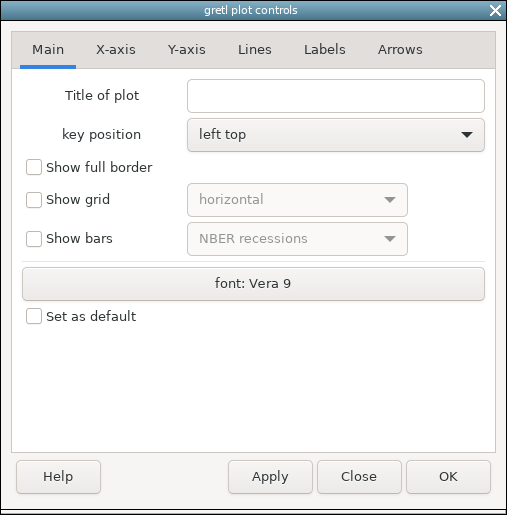
\includegraphics[scale=0.75]{figures/plot_control}
  \end{center}
  \caption{Finestra di modifica dei grafici gnuplot di gretl}
  \label{fig-plot}
\end{figure}


\section{Boxplot}
\label{sect-boxplots}

I grafici boxplot non vengono generati con gnuplot, ma da \app{gretl}
stesso.

Questi grafici (da Tukey e Chambers) mostrano la distribuzione di una
variabile. La ``scatola'' centrale (box) racchiude il 50 per cento
centrale dei dati, ossia � delimitata dal primo e dal terzo quartile. I
``baffi'' (whiskers) si estendono fino ai valori minimo e massimo. Una
linea trasversale sulla scatola indica la mediana.  

Nel caso dei grafici a tacca (``notches''), una tacca indica i limiti
dell'intervallo di confidenza approssimato al 90 per cento per la
mediana, ottenuto col metodo bootstrap (se la serie dei dati � molto
lunga, potrebbe essere necessario un po' di tempo).

Facendo clic nella finestra del boxplot si ottiene un men� che
permette di salvare il grafico come file encapsulated postscript (EPS)
o come file postscript a piena pagina. Se si usa il sistema X Window �
anche possibile salvare il grafico come file XPM, mentre in MS Windows
� possibile copiarlo negli appunti in formato bitmap. Il men� d� anche
la possibilit� di mostrare un riepilogo in cinque numeri (minimo,
primo quartile, mediana, terzo quartile, massimo) e un intervallo di
confidenza per la mediana, se il boxplot � del tipo ``a tacca''.

Alcuni dettagli del funzionamento dei boxplot di gretl possono essere
controllati attraverso un file testuale chiamato \verb+.boxplotrc+,
che viene cercato, nell'ordine, nella directory di lavoro attuale,
nella directory home dell'utente (che corrisponde alla variabile
d'ambiente HOME) e nella directory utente di gretl (scelta attraverso
il comando ``Strumenti, Preferenze, Generali...'').  Tra le opzioni che
possono essere specificate in questo modo ci sono: il carattere da
usare per l'output in postscript (deve essere un nome di font
postscript valido; il valore predefinito � Helvetica), la dimensione
del carattere in punti (sempre per l'output in postscript; il valore
predefinito � 12), i valori minimo e massimo per l'asse y, la
larghezza e l'altezza del grafico in pixel (valori predefiniti: 560 x
448), se occorre mostrare anche i valori numerici per i quartili e la
mediana (l'impostazione predefinita non li mostra) e se occorre
indicare separatamente gli outlier, ossia i punti che distano pi� di
1.5 volte il range interquartile dalla scatola centrale
(l'impostazione predefinita non li mostra). Ecco un esempio:

\begin{code}
font = Times-Roman
fontsize = 16
max = 4.0
min = 0
width = 400
height = 448
numbers = %3.2f
outliers = true
\end{code}

Sulla penultima riga, il valore associato a \verb+numbers+ � una
stringa di formato ``printf'' come quelle usate nel linguaggio di
programmazione C; se viene specificata, controlla il modo in cui
vengono mostrati la mediana e i quartili accanto al boxplot,
altrimenti questi valori non vengono mostrati. Nell'esempio, i valori
verranno mostrati usando 3 cifre in totale e 2 cifre di precisione
dopo il punto decimale.

Non occorre specificare tutte le opzioni, n� importa l'ordine in cui
vengono specificate. Le righe che non seguono la struttura ``variabile
= valore'' vengono ignorate, cos� come le righe che iniziano con il
carattere cancelletto, \verb+#+.  

Dopo ogni variabile specificata nel comando boxplot � possibile
inserire un'espressione booleana tra parentesi per limitare il
campione da utilizzare per la variabile in questione, avendo cura di
inserire uno spazio tra il nome (o il numero) della variabile e
l'espressione. Si supponga di avere una variabile \verb+salario+ con
gli stipendi di uomini e donne, e una variabile dummy \verb+GENERE+
che vale 1 per gli uomini e 0 per le donne. In questo caso � possibile
disegnare dei boxplot comparativi usando il seguente comando nella
finestra di dialogo:
      
\begin{code}
salario (GENERE=1) salario (GENERE=0)
\end{code}


%%% Local Variables: 
%%% mode: latex
%%% TeX-master: "gretl-guide-it"
%%% End: 

